\documentclass{llncs}
%
\usepackage{subcaption,graphicx,hyperref,listings}
\captionsetup{compatibility=false}
\renewcommand{\sectionautorefname}{\S}
\renewcommand{\subsectionautorefname}{\S}
\renewcommand{\subsubsectionautorefname}{\S}
\lstset{
	basicstyle=\scriptsize\ttfamily,
	breaklines=true,
	breakatwhitespace=true,
	escapechar=\%,
	numbers=left,
	tabsize=2,
	xleftmargin=2em
}
\renewcommand{\topfraction}{0.85}
\renewcommand{\textfraction}{0.1}
\renewcommand{\floatpagefraction}{0.85}
%
\begin{document}
%
\mainmatter              % start of the contributions
%
\title{Using Diversity to Harden Multithreaded Programs Against Exploitation}
%
\author{
	%Anonymized for Review
	David M. Tagatac\inst{1}
	\and
	Michalis Polychronakis\inst{2}
	\and
	Salvatore J. Stolfo\inst{1}
}
%
\institute{
	%Do not Distribute
	Columbia University in the City of New York, NY 10027\\
	\{\texttt{dtagatac}, \texttt{sal}\}\texttt{@cs.columbia.edu}
	\and
	Stony Brook University, Stony Brook, NY 11794\\
	\texttt{mikepo@cs.stonybrook.edu}
}

\maketitle              % typeset the title of the contribution

\begin{abstract}
Multithreaded programming is here to stay, and concurrency bugs are the focus of a growing number of cyberattacks.
While most defensive efforts against such attacks seek to identify bugs during
debugging, an alternative method seeks to make exploitation harder without the
need to first identify the bugs---or even the fact that there are any.
Time randomization introduces more diversity among instances of the same software.
In much the same way that ASLR-induced diversity in memory locations thwarts attacks crafted for specific addresses, time randomization-induced diversity in thread timing aims to thwart concurrency attacks crafted for specific vulnerability windows.

We study three implementations of time randomization, all using the injection of NOPs to alter program timing.
Their application to two real-world concurrency bugs results in a marked increase in the cost to exploit those bugs.
After demonstrating the effectiveness of the method, especially when NOPs are injected before library function calls following synchronization points, methods for improving the efficiency of this defense against concurrency attacks in future research are proposed.

\keywords{time randomization, concurrency bugs, software diversity}
\end{abstract}
%
\section{Introduction}
With the pervasiveness of multicore architectures, multithreading is an important - and often necessary - tool when programming for performance.
However, programming with multiple threads is generally more difficult than programming for serial execution.
Each thread has the potential to contain any bug of a serial program, and on top of that, the uncertain interleaving of concurrent threads has the potential for concurrency bugs (e.g. data races).

Partial taxonomies of concurrency bugs have been constructed \cite{Farchi2003, Lu2008}, and it has been demonstrated that attacks on buggy multithreaded programs are a real concern \cite{Yang2012}.
Much of the effort in combating this threat has gone into tools and systems which detect data races in order to aid debugging \cite{Savage1997, Flanagan2004, Laadan2011, Pratikakis2011, Kasikci2013}.
An alternative approach is to guide multithreaded programs into memoized synchronization schedules \cite{Cui2010}.
This approach does not dwell on race detection, but rather on removing the nondeterminism from the portions of multithreaded programs where races are most likely.
However, schedule memoization in its most automated form is still susceptible to attack whenever the attacker can trigger a different schedule by changing the input.

We address the threat of concurrency attacks from yet another angle: automated software diversity.
Software homogeneity is dangerous in that it provides economies of scale to attackers \cite{Geer2003b}.
The relatively high cost of constructing an exploit for one bug is ameliorated by the opportunity to reuse that same exploit on every identical instance of the software.
As a result, automated software diversity is an active area of research for software in general \cite{Larsen2014}.
Concurrency vulnerabilities subject a homogenous world of software to the same dangers for the same reasons.

Our contribution is the experimental analysis of three implementations of automated software diversity through instruction level randomization via NOP injection:
\begin{enumerate}
	\item Injection of random-length NOP loops before every library function call.
	\item Injection of random-length NOP loops before every library function call immediately preceding a synchronization mechanism.
	\item Injection of random-length NOP loops before every library function call immediately following a synchronization mechanism.
\end{enumerate}

We find the first and third implementations above to be effective in increasing exploit cost on two real-world concurrency bugs.
However, the overhead is too high to recommend these implementations as practical solutions.
We propose future directions for achieving the benefits of this defense without overhead, or with more tolerable overhead.

\section{Time Randomization}
\subsection{Threat Model}\label{threat-model}
The type of attack that time randomization seeks to thwart has the following properties:
\begin{itemize}\addtolength{\itemsep}{-.35\baselineskip}
	\item The attack targets a concurrency bug.
	\item The attacker can gain knowledge about the relative timing between two
  or more threads relevant to the bug.
	\item The attacker leverages this knowledge to craft the attack.
\end{itemize}
Note that there are many ways to gain knowledge about relative thread timing, including results from fuzzing experiments.
In the case that the fuzzing is done on a binary, it may not even be obvious how many threads are involved.
Nevertheless, positive fuzzing results can be considered knowledge about relative thread timing which can then be used to craft an attack.

As an example, consider the following scenario:
A remote attacker is communicating with some server software, and has somehow become aware of a concurrency bug in that software.
They have devised a way to exploit the bug, which includes a method for inducing a buggy thread interleaving.
For concreteness, let's assume that the bug is exposed when a save operation
is attempted by one thread during the critical section of another save
operation in another thread (e.g., after some checking has been done, but before the results have been used, sometimes referred to as a time of check to time of use attack).
If the server immediately spawns threads to execute save operations in response to client requests, the attacker's work consists of identifying the proper delay between two save threads such that the critical sections intersect.
The critical sections in this context are sometimes referred to as a vulnerability window~\cite{Yang2012}.

If the server software is available to the attacker, they can simply study it on a similar system (which they control) to determine the appropriate delay required to expose the bug.
Armed with this knowledge, they stand a good chance of exploiting the bug on the target system by sending requests with the same delay.
\begin{figure*}
	\centering
	\begin{subfigure}{\columnwidth}
		\fbox{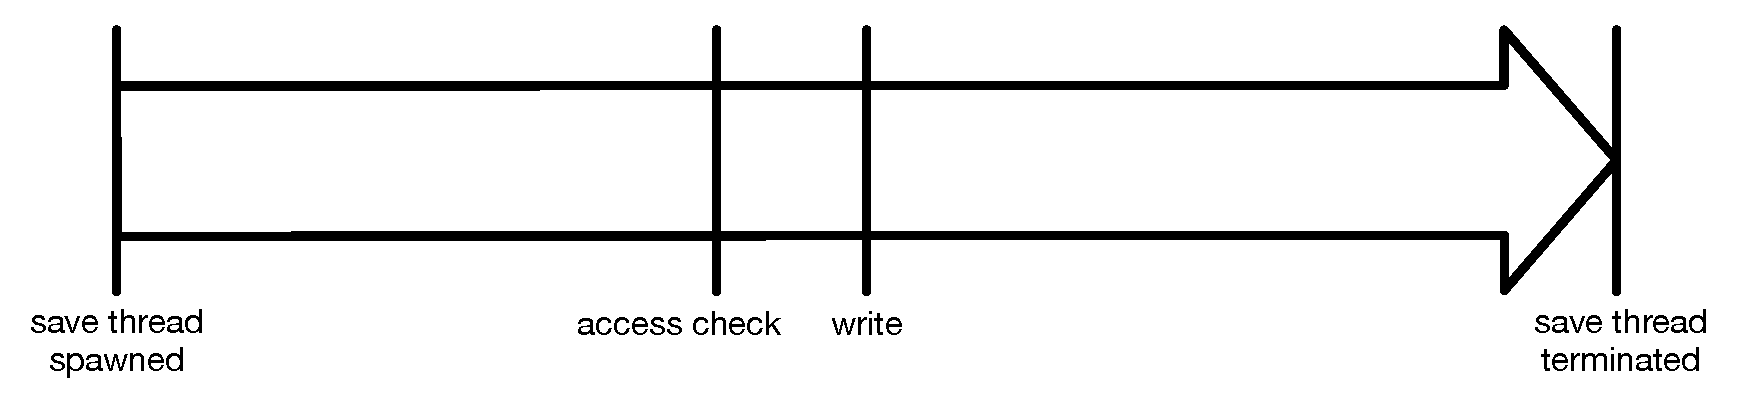
\includegraphics[width=.95\textwidth]{figures/save_op}}
		\caption{A single save operation thread.}
		\label{fig_save_op}
	\end{subfigure}
	\begin{subfigure}{\columnwidth}
		\fbox{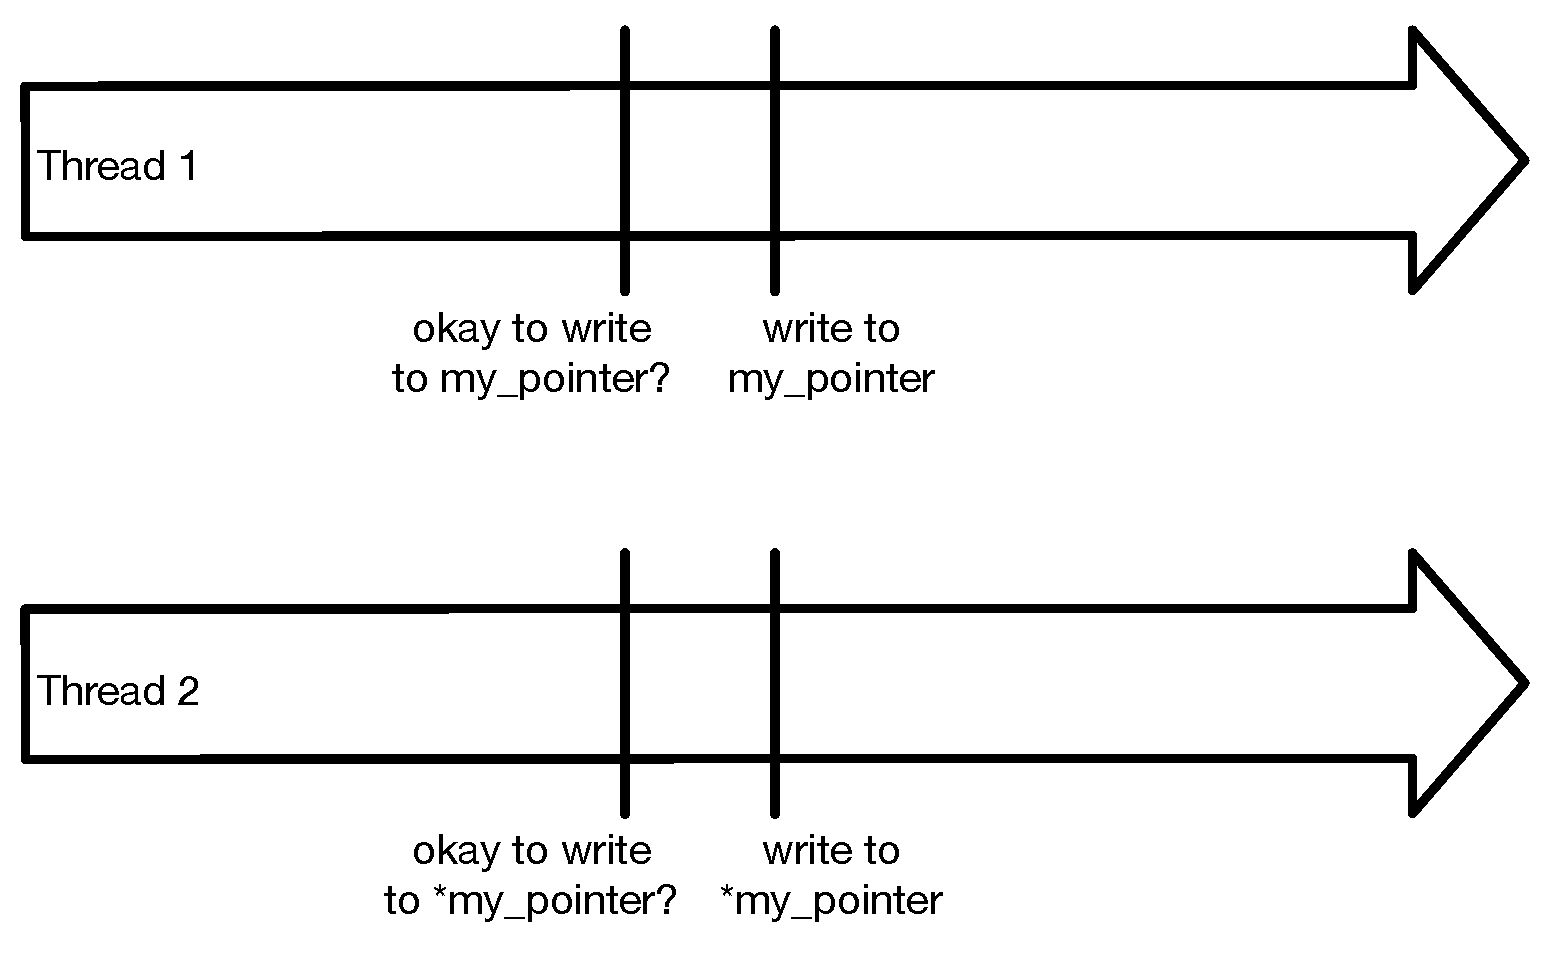
\includegraphics[width=.95\textwidth]{figures/two_threads}}
		\caption{Two save operation threads.}
		\label{fig_two_threads}
	\end{subfigure}
	\begin{subfigure}{\columnwidth}
		\fbox{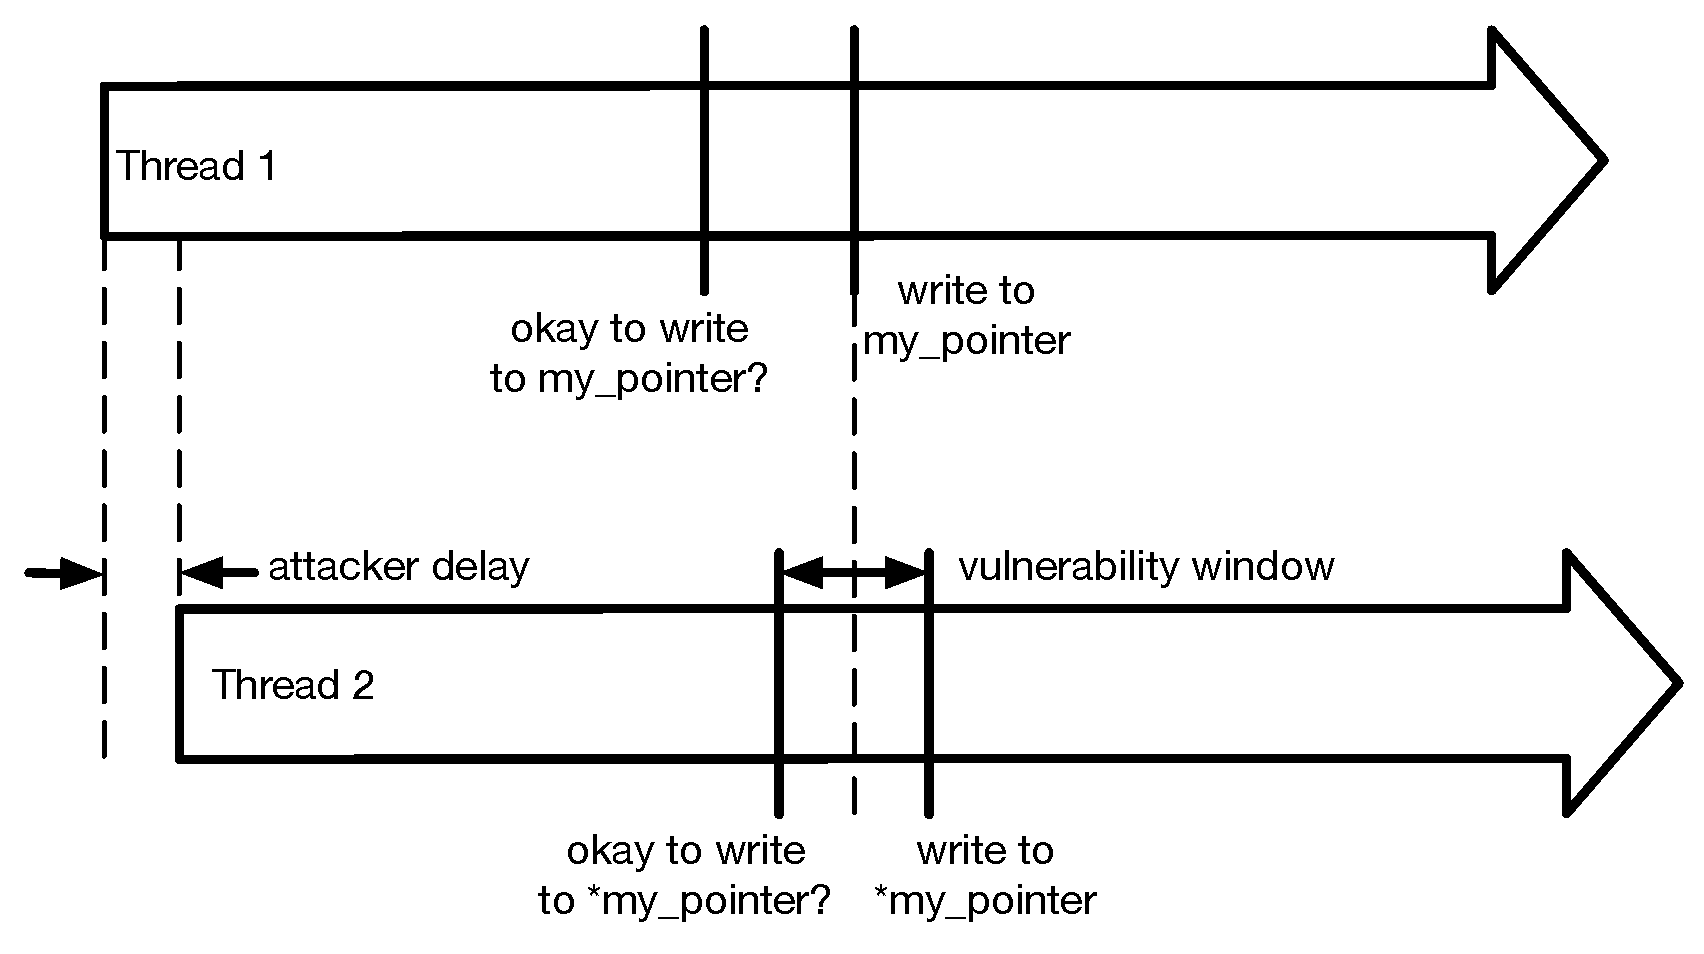
\includegraphics[width=.95\textwidth]{figures/attack}}
		\caption{A constructed attack using timing knowledge.}
		\label{fig_attack}
	\end{subfigure}
	\begin{subfigure}{\columnwidth}
		\fbox{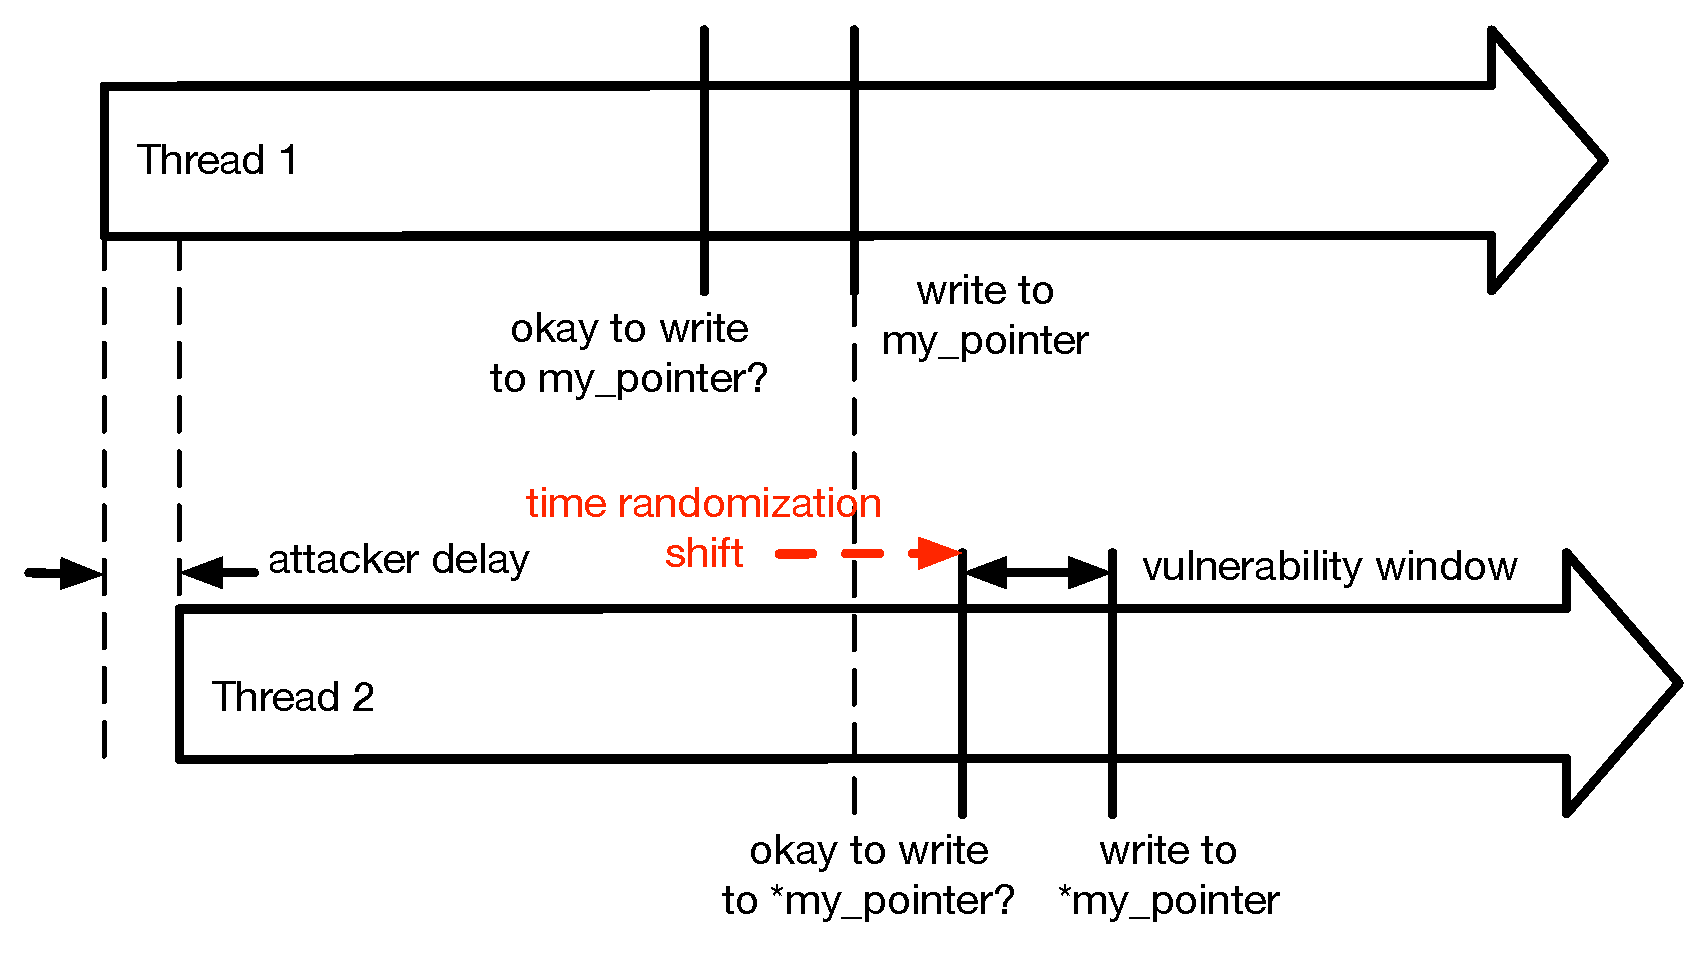
\includegraphics[width=.95\textwidth]{figures/thwart}}
		\caption{An example result of time randomization.}
		\label{fig_thwart}
	\end{subfigure}
	\caption{A pictorial representation of the example concurrency attack described in \autoref{threat-model}.}
	\label{fig_exploitation}
\end{figure*}
\subsection{Implementation}\label{implementation}
Time randomization, the randomization of synchronization schedules and thread interleavings, as well as the relative timing between and among threads, aims to make this type of attack much harder.
By making the relative timing between threads less predictable, the cost of carrying out the attack above is dramatically increased.
Figure~\ref{fig_exploitation} presents a graphical explanation of this attack and one possible result of time randomization that would cause it to fail.

Figure~\ref{fig_save_op} depicts a single save operation thread with two significant points---an access check where the thread checks whether the requestor has the proper access rights to make the requested change, and a write where the requested change is made (assuming the access check succeeds).
Figure~\ref{fig_two_threads} shows two save operation threads.
Thread 1 is saving to the (poorly designed) global variable \texttt{my\_pointer}.
Thread 2 is saving to the memory location indicated by \texttt{my\_pointer}.
We can see the makings for a TOCTOU attack here---if \texttt{my\_pointer} points to a memory location to which the attacker has access, the check in Thread 2 will succeed; but if Thread 1 modifies \texttt{my\_pointer} to point to another memory location to which the attacker should not have access before Thread 2 writes, Thread 2 will write to that memory location.
An attacker has thus achieved privilege escalation.
In fact, if the thread timing (i.e., the timing between thread spawn and the significant points labeled in Figure~\ref{fig_save_op}, and the relative timing between Thread 1 and Thread 2) are predictable, the attacker can study that thread timing on another system that they control (Figure~\ref{fig_attack}).
They can then determine an appropriate delay between spawning Thread 1 and Thread 2 such that the write to \texttt{my\_pointer} by Thread 1 falls inside the vulnerability window of Thread 2.
Finally, Figure~\ref{fig_thwart} shows an example result of time randomization.
Here, time randomization has shifted the vulnerability window of Thread 2 with respect to the write by Thread 1 such that the delay calculated by the attacker in Figure~\ref{fig_attack} no longer aligns the two.
This result can be achieved, for example, by a time randomization transformation which adds a delay between the spawning of Thread 2 and the access check by Thread 2.
Note that a delay between the spawning of Thread 1 and the write by Thread 1 would also cause the write to miss the vulnerability window in Thread 2.

Of the various software diversity transformations which have been studied~\cite{Larsen2014}, the ones which are most applicable to time randomization are those which
\begin{itemize}\addtolength{\itemsep}{-.35\baselineskip}
	\item add delays to a thread or threads, and those which
	\item reorder something such that thread interleaving is affected.
\end{itemize}
The first category is almost always possible, as adding delays rarely breaks programs.
However, an obvious drawback to this approach is loss of performance, and this drawback must be weighed against the benefits of the transformation.
In the second case, the ``something'' reordered can be at any granularity (instruction level, function level, program level, etc.) so long as thread interleaving is affected.
These types of transformations are less likely to have performance costs, but they are more likely to break the correctness of programs.
This work studies three transformations in the first category.

The three transformations for introducing automated diversity explored in the context of concurrency attacks in this work consist of interposing external library calls~\cite{Conrad2009} made by the software to be protected each with random numbers of inline assembly NOP instructions.
This was accomplished by first specifying a max delay (per interposition).
Then, for each of the external library functions chosen for interposition, a random integer between zero and the max delay was selected.
Finally, that number was used as the loop limit on a loop of assembly NOPs for that external library function.
The interpositions of the NOP loops were compiled into a dynamic library file, and that file was specified to be preloaded with the LD\_PRELOAD environment variable.

The three transformations vary only in the way that the library functions are chosen for interposition.
The first transformation chooses all external library function calls indiscriminately, while the other two use synchronization mechanisms to indicate locations where delays may have the greatest effect on relative thread timing.
In all transformations, \texttt{ltrace}~\cite{cespedesltrace} is run on the unmodified program to be protected while it is being subjected to an exploit attempt.
Using the log from that ltrace run,
\begin{description}\addtolength{\itemsep}{-.35\baselineskip}
	\item[T1] the first transformation chooses every external library function call for interposition,
	\item[T2] the second transformation chooses every external library function call immediately preceding a synchronization mechanism, and
	\item[T3] the third transformation chooses every external library function call immediately following a synchronization mechanism.
\end{description}
(Hereafter, these transformations are referred to as \textbf{T1}, \textbf{T2}, and \textbf{T3}.)
Functions were only excluded in the rare cases that the function takes a
variable argument list, or interposing the function interferes with the
interposition method itself (e.g., \texttt{sigsetjmp}).
Both cases are unsuitable for the interposition method used in this work.
As all of the experiments were conducted on Linux, ``synchronization
mechanisms'' were generally identified as \texttt{pthread} function calls, except for the case of Libvirt which redefines its own synchronization mechanisms.

In addition to the question of the proper diversity transformation, there is also the question of when (or how often) to diversify.
We do not address the latter here, except insofar as the transformations tested here dictate that the diversification must be done prior to load time (so that the interposition library is available for preloading).
As the randomization processes \textbf{T1}-\textbf{T3} require considerable computation, diversification at \textit{each} load time is likely infeasible.
However, one could certainly imagine these transformations being applied at install time, and even possibly at each reboot.

\section{Experimental Design}
To test both the efficacy and the performance of time randomization as a mechanism to thwart concurrency bug exploitation, we applied time randomization to two canonical and two real concurrency bugs.
\subsection{Real Bug: Libsafe CVE-2005-1125}
Libsafe \cite{Tsai2001} is a library which protects processes against the
exploitation of buffer overflow vulnerabilities in process stacks, as well as
format string vulnerabilities.  It does this by intercepting all calls to C
standard library functions known to be vulnerable, and then running ``safe'' versions of those functions which issue warnings about exploit attempts before exiting without allowing the exploits to succeed.

A static global variable `dying' is used in Libsafe to indicate when an unsafe action has already been detected, and Libsafe is issuing warnings and exiting.  In this case, Libsafe stops checking for new exploit attempts.  However, this variable is not protected by any synchronization mechanisms, so in the case of a multithreaded program, the following sequence of events is possible:
\begin{enumerate}
	\item Thread A attempts an exploit.
	\item The exploit is caught by Libsafe, the `dying' flag is set, and Libsafe begins the warning and exit procedure.
	\item Thread B is scheduled, and attempts another exploit before Libsafe has exited thread A.
	\item Because the `dying' flag is set, thread B's exploit is not caught by Libsafe, and it succeeds.
\end{enumerate}
The proof-of-concept exploit (Figure \ref{fig_poc})\cite{Bugtraq13190} often realizes the above sequence of events, effectively bypassing Libsafe.
\begin{figure}
	\lstinputlisting{libsafe-PoC.c}
	\caption{The proof of concept exploit for concurrency bug CVE-2005-1125 \cite{CVE-2005-1125}.  Both functions \texttt{func1} and \texttt{func2} attempt to overflow buffers in their own stack frames.  Either function running alone would be caught by Libsafe at the illegal calls to \texttt{strcpy}, but when run in parallel, the concurrency bug may allow one call to \texttt{strcpy} to succeed.}
	\label{fig_poc}
\end{figure}

Time randomization was applied to Libsafe as described in \autoref{automated-diversity}.
The time required to make a (legal) \texttt{strcpy} function call (using Libsafe and averaged over 10,000,000 \texttt{strcpy} calls), and the proof of concept exploit success rate were measured for several randomizations for each max delay, where max delay was varied from 0 to 50,000.
Automated diversity implementations 2 and 3 were a special cases in that only one external library function was identified as immediately preceding a synchronization mechanism and only one external library function was identified as immediately following a synchronization mechanism.
In these cases, we were able to exactly characterize the effects of NOP injection as a function of the number of NOPs injected into that function.
\subsection{Real Bug: Libvirt CVE-2014-1447}
Libvirt \cite{libvirt} is a toolkit for interacting with virtual machines and hypervisors.
This toolkit consists, in part, of a daemon `libvirtd' which listens for and
responds to virtual machine management requests (e.g., to connect to a remote host, or shutdown a VM).

Prior to version 1.2.1, the Libvirt daemon suffered from concurrency bug CVE-2014-1447 which allows an unauthenticated client to crash the daemon with seemingly innocuous requests to connect to a host.
After receiving a request from a client to open a connection, the daemon spawns a thread to open and maintain that connection.
The spawned thread will eventually dereference a pointer called
``client->keepalive'' as part of opening the connection.
However, during this vulnerability window, the client may close the
connection, which the daemon will handle in the main thread by (among other
things) setting ``client->keepalive'' to NULL.
Then when the spawned thread dereferences this pointer, the daemon crashes. \cite{RHELbug1047577}

The Libvirt developers' proof of concept makes two changes to Libvirt in order to reliably reproduce this bug.
First, the client is modified to exit as soon as it has requested a connection.
Second, the daemon is modified to sleep in threads spawned to open new
connections, before dereferencing the ``client->keepalive'' pointer.
The first modification is within an attacker's ability, in our threat model.
However, the second modification requires control of the daemon, which we assume the attacker does not yet have.
An alternate exploit requiring only the first modification was applied to Libvirt 0.9.8.
In this alternate exploit, the client opens (and closes) as many connections as it can until the daemon crashes.
Without modification to the daemon, this alternate exploit reliably reproduced the bug and crashed the daemon.

Time randomization was applied to the Libvirt daemon as described in \autoref{automated-diversity}.
The time required to open and close a connection properly (with the unmodified client averaged over 10,000 sequential connections) was measured, and the time required for the alternate exploit described above to crash the daemon was measured five times for a single randomization for each max delay, where max delay was varied from 0 to 1,000,000.
All exploit attempts were interrupted and considered failed attempts after ten minutes if they did not succeed before then.
\subsection{Canonical Bug: Nonatomic Operations Assumed to be Atomic}
Farchi et al. presented a partial concurrency bug taxonomy \cite{Farchi2003}, and Lu et al. later showed that in a narrow study of real world concurrency bugs, the vast majority are one of two types \cite{Lu2008}:
\begin{enumerate}
	\item Atomicity Violation: The desired serializability among multiple memory accesses is violated.
	\item Order Violation: The desired order between two memory accesses is flipped.
\end{enumerate}
To test time randomization on the first type, a simple concurrency bug was
constructed mimicking a ``nonatomic operations assumed to be atomic'' programmer error \cite{Farchi2003}.
In particular, in Python, the statement \texttt{x+=1} is nonatomic, but may be mistaken to be atomic due to its compact syntax.
Our simple concurrency bug (Figure \ref{fig_nonatomic}) contains a loop that expects this statement (unprotected by synchronization mechanisms) to always increment \texttt{x} by one.
An ``exploit'' runs in a separate thread, modifying \texttt{x} periodically.
The exploit succeeds when the statement \texttt{x+=1} in the first thread fails to increment \texttt{x} by exactly one.
In other words, the exploit thread modifies \texttt{x} within the vulnerability window (between when \texttt{x} is read from memory, and when it is written back to memory by the first thread).
\begin{figure}
	\lstinputlisting{nonatomic.py}
	\caption{A canonical atomicity violation concurrency bug.  The \texttt{xplusplus} function assumes the nonatomic statement \texttt{x+=1} to be atomic.  The \texttt{fuzzer} function, run in a separate thread, attempts to exploit this assumption by modifying \texttt{x} within the vulnerability window (between when \texttt{x} is read from memory, and when it is written back to memory).}
	\label{fig_nonatomic}
\end{figure}

Time randomization was applied to this bug as described in \autoref{automated-diversity}.
The time required to complete the operations encoded in the statement \texttt{x+=1} (averaged over 10,000,000 sequential executions of that statement), and the number of exploit loop iterations required to succeed were measured for a single randomization for each max delay, where max delay was varied from 0 to 1,000,000.
%TODO: discuss sleep in exploit thread
%Knowledge of the time required to execute the instructions encoded by the
%statement \texttt{x+=1} can be utilized by the exploit thread to achieve
%``exploitation'' in fewer loops.
%Note in Figure \ref{fig_nonatomic} that the exploit thread is identical to the buggy thread except for a \texttt{sleep()} at the beginning of each loop iteration.
%The \texttt{sleep()} has a duration of half of the time required to complete the statement \texttt{x+=1}.
%This sleep can be thought of as shifting the exploit thread loop (\texttt{fuzz}) with respect to the buggy thread loop (\texttt{xplusplus}).
%In the best case (for the exploit), this corresponds to altering \texttt{x} at intervals of half of the vulnerability window (modulo the time for one loop iteration).
%Of course the shift is imperfect due to the nondeterminism in thread scheduling, but the effect is significant in practice.
%The table below shows the average number of `exploit loop' iterations required to alter \texttt{x} within the vulnerability window over ten runs.
%This measurement is repeated for values of \texttt{HALF} equal to (0, 2.8e-05, 2.8e-04, 2.8e-03, and 2.8e-02), where the measured time to complete the statement \texttt{x+=1} on the test system was approximately
%\subsection{Canonical Bug: Order Violation}
%TODO

\section{Results}\label{results}
We evaluated \textbf{T1}-\textbf{T3} on Libsafe CVE-2005-1125, \textbf{T2} and \textbf{T3} on Libvirt CVE-2014-1447, and \textbf{T3} on the canonical ``nonatomic operations assumed to be atomic'' bug.
For each evaluation, exploit cost or exploit success rate was evaluated for each of many applications of the transformation under study.
The exploit cost or success rate was then compared to either the microbenchmark overhead, or the number of NOPs injected, as appropriate for each experiment.
Libsafe and ``nonatomic operations assumed to be atomic'' experiments were run on a dedicated dual core 3.4GHz Pentium D running Debian.
Libvirt experiments were run on a 2.8GHz dual-socket hex-core Intel Xeon with 24 hyper-threading cores running Ubuntu.
In all figures, the horizontal red line indicates the average measurement for the unmodified bug (without time randomization).
The results vary somewhat widely with the bug analyzed and the automated diversity transformation used.
A summary of the results in this section is given in Table \ref{tab_results}.
\begin{table}
	\centering
	\begin{tabular}{ | p{0.6in} | p{0.6in} | p{0.6in} | p{0.6in} | }
	\hline
	Bug & Transfor\-mation Applied & Time Randomization Effective? & Figure \\ \hline
	\hline
	Libsafe & \textbf{T1} & Yes & \ref{fig_libsafe-all}\&\ref{fig_libsafe-all-zoom} \\ \hline
	Libsafe & \textbf{T2} & No & \ref{fig_libsafe-pre} \\ \hline
	Libsafe & \textbf{T3} & Yes & \ref{fig_libsafe-post} \\ \hline
	Libvirt & \textbf{T2} & No & \ref{fig_libvirt-pre} \\ \hline
	Libvirt & \textbf{T3} & Yes & \ref{fig_libvirt-post} \\ \hline
	Canonical Atomicity Violation & \textbf{T3} & No & \ref{fig_nonatomic-post} \\ \hline
	\end{tabular}
	\caption{A summary of the results in \autoref{results}.}
	\label{tab_results}
\end{table}

Applying transformation 1 (interposition of all external library function calls) to Libsafe resulted in a dramatic decrease in exploit success rate with increasing microbenchmark overhead (Figures \ref{fig_libsafe-all} and \ref{fig_libsafe-all-zoom}).
Between 1x overhead and 12x overhead, no randomizations resulted in less than a 5\% success rate.
Between 20x and 25x overhead, 27.5\% of randomizations resulted in less than a 5\% exploit success rate.
Between 40x and 45x overhead, 61.5\% of randomizations resulted in less than a 5\% exploit success rate.
Beyond 1,040x overhead, 100\% of randomizations resulted in less than a 5\% exploit success rate.
\begin{figure}
	\centering
	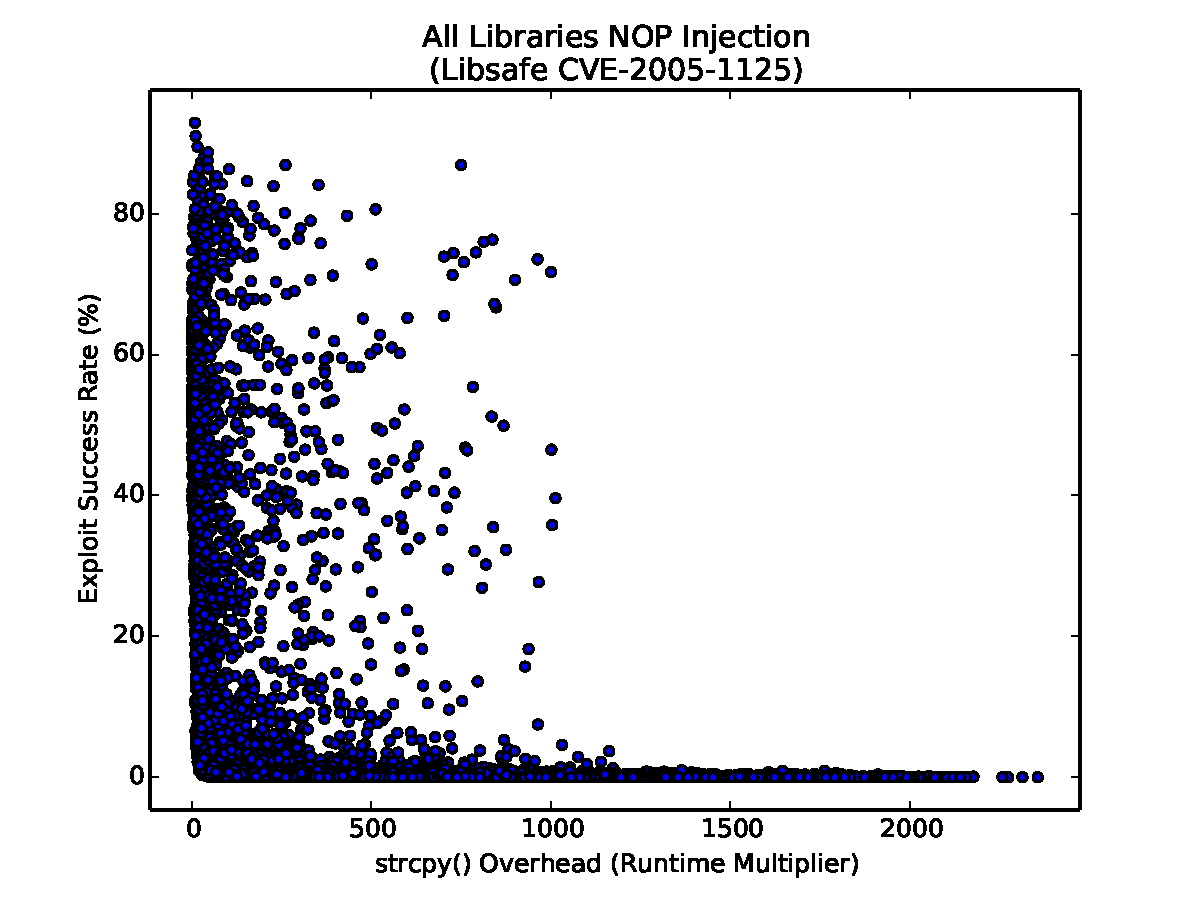
\includegraphics[width=.75\columnwidth]{figures/libsafe-all}
	\caption{Exploit success rate as a function of the microbenchmark after applying \textbf{T1} to Libsafe with concurrency bug CVE-2005-1125.}
	\label{fig_libsafe-all}
\end{figure}
\begin{figure}
	\centering
	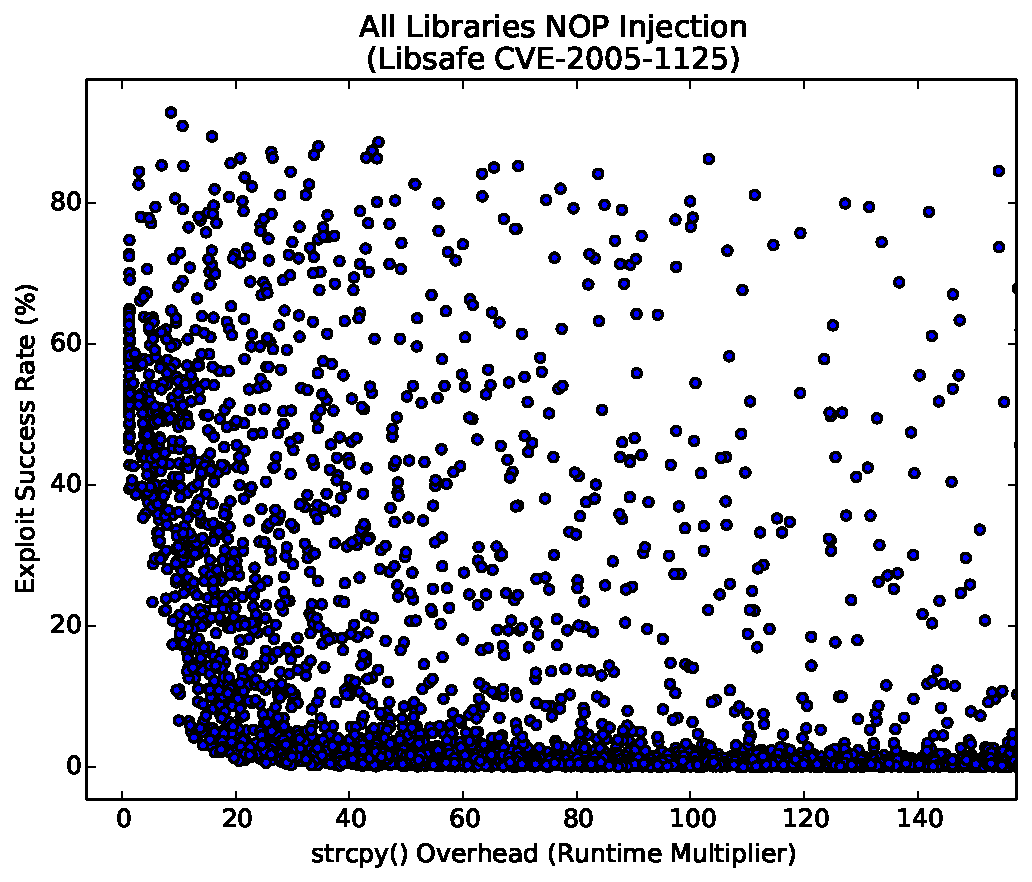
\includegraphics[width=.75\columnwidth]{figures/libsafe-all-zoom}
	\caption{
		Exploit success rate as a function of the microbenchmark after applying \textbf{T1} to Libsafe with concurrency bug CVE-2005-1125 (a zoom-in of Figure \ref{fig_libsafe-all}).
		There is a clear inverse correlation between microbenchmark overhead and exploit success rate.
	}
	\label{fig_libsafe-all-zoom}
\end{figure}

Applying \textbf{T2} to Libsafe had no noticeable effect on exploit success rate (Figure \ref{fig_libsafe-pre}) or microbenchmark overhead.
\begin{figure}
	\centering
	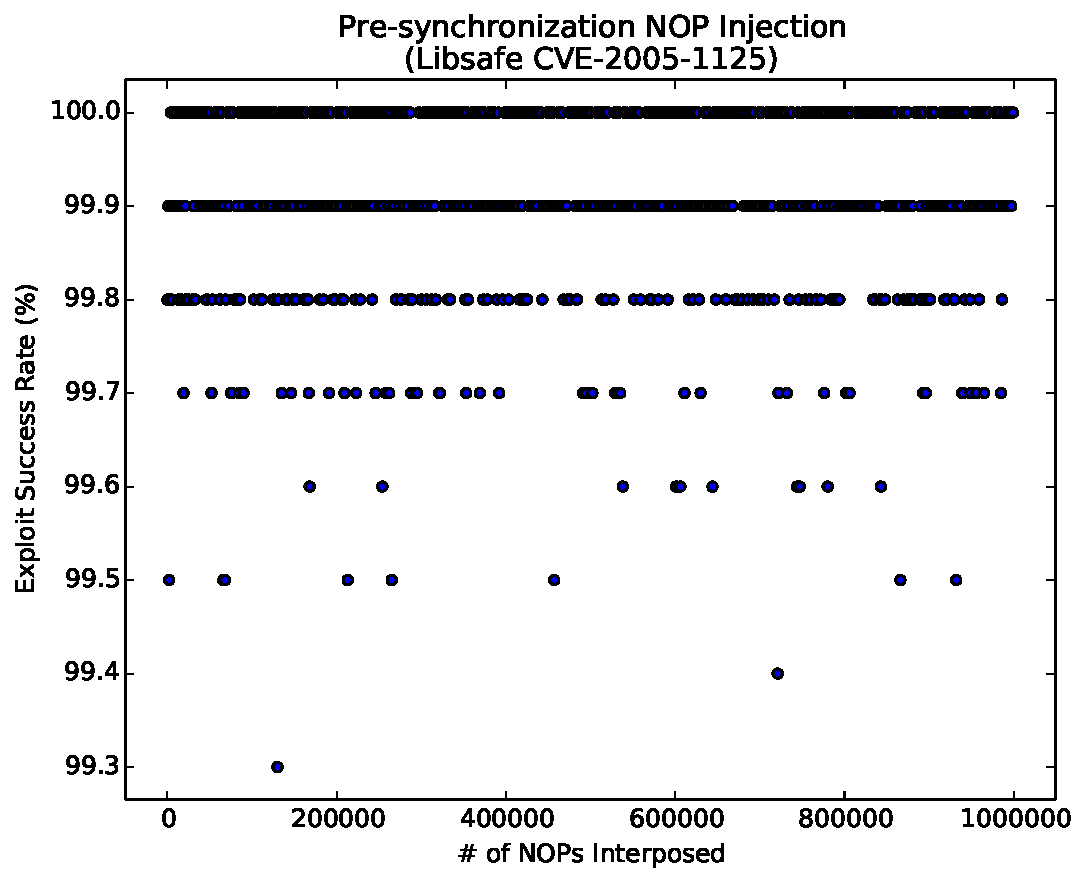
\includegraphics[width=.75\columnwidth]{figures/libsafe-pre}
	\caption{
		Exploit success rate as a function of the microbenchmark after applying diversity \textbf{T2} to Libsafe with concurrency bug CVE-2005-1125.
		This transformation does not appear to have an effect on exploit success rate for this bug.
	}
	\label{fig_libsafe-pre}
\end{figure}

Applying \textbf{T3} to Libsafe had a very marked effect on exploit success rate (Figure \ref{fig_libsafe-post}).
In particular, exploit success rate remains high for low numbers of NOPs.
Then, for inserted NOP loops of lengths greater than 200,000, exploit success rate begins to drop.
For inserted NOP loops of lengths between 250,000 and 350,000, exploit success rate fluctuates between 35\% and 65\%.
Finally, for inserted NOP loops of lengths greater than 350,000, exploit rates drop even further, and beyond loop-lengths of 390,000 NOPs, all interpositions resulted in exploit rates less than 0.5\%.
\begin{figure}
	\centering
	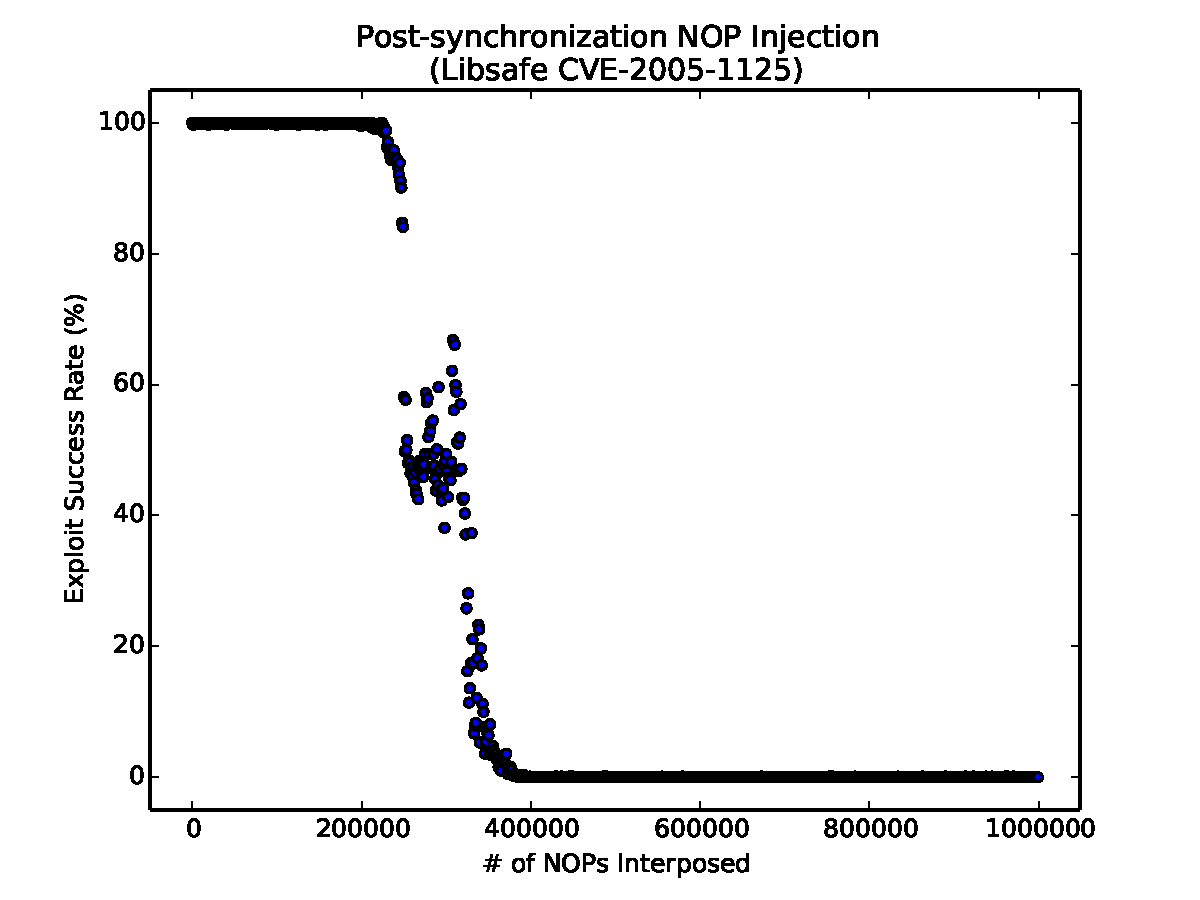
\includegraphics[width=.75\columnwidth]{figures/libsafe-post}
	\caption{
		Exploit success rate as a function of the number of NOPs injected after applying \textbf{T3} to Libsafe with concurrency bug CVE-2005-1125.
		A very clear inverse correlation between NOP loop length and exploit success rate is shown.
	}
	\label{fig_libsafe-post}
\end{figure}

\begin{figure}
	\centering
	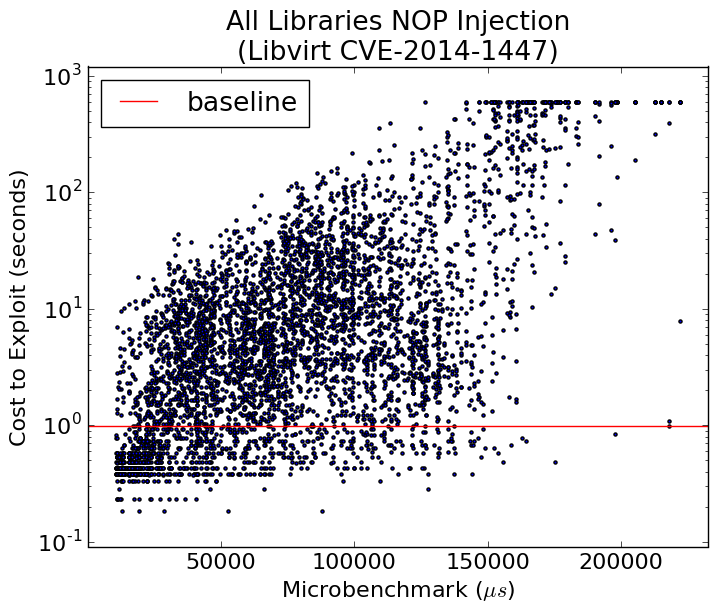
\includegraphics[width=.75\columnwidth]{figures/libvirt-all}
	\caption{
		Exploit cost (in time) as a function of the microbenchmark after applying \textbf{T1} to Libvirt with concurrency bug CVE-2014-1447.
	}
	\label{fig_libvirt-all}
\end{figure}

Applying \textbf{T2} to Libvirt did not seem to have much of an effect on exploit cost.
The characteristic of most exploit attempts succeeding quickly, and a few taking much longer appears to be consistent throughout the range of microbenchmark values recorded (Figure \ref{fig_libvirt-pre}).
\begin{figure}
	\centering
	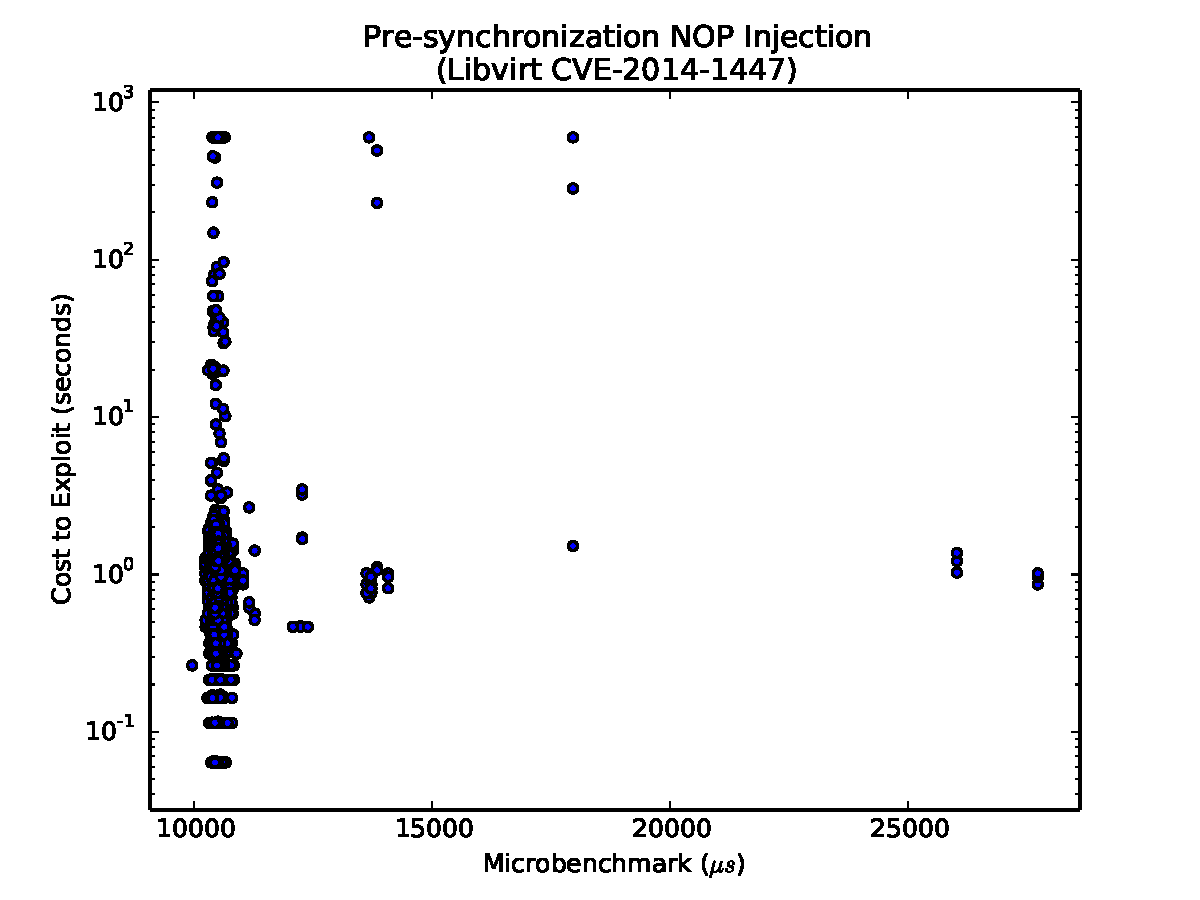
\includegraphics[width=.75\columnwidth]{figures/libvirt-pre}
	\caption{
		Exploit cost (in time) as a function of the microbenchmark after applying \textbf{T2} to Libvirt with concurrency bug CVE-2014-1447.
		This transformation does not appear to have an effect on exploit success rate for this bug.
	}
	\label{fig_libvirt-pre}
\end{figure}

\textbf{T3} applied to Libvirt, as in the case of Libsafe, had a significant effect on exploit cost.
For microbenchmark connection times of less than 10 milliseconds, less than 4\% of exploit attempts took longer than the baseline exploit time of 1.11 seconds, where the baseline exploit time was obtained for a Libvirt daemon without any time randomization.
By contrast, for microbenchmark times of greater than 10 milliseconds, nearly 85\% of exploit attempts took longer than the baseline exploit time.
Looking at the graph (Figure \ref{fig_libvirt-post}), we can see a similar shape to the one obtained when applying \textbf{T2} to Libvirt - the bifurcation between exploit attempts that succeed quickly within seconds, and those which take hundreds of seconds to succeed.
However, after applying automated \textbf{T3}, a significantly greater proportion of exploit attempts fell into the second branch of that bifurcation, taking hundreds of seconds to succeed, or failing to succeed within ten minutes (and being categorized as failed attempts).
\begin{figure}
	\centering
	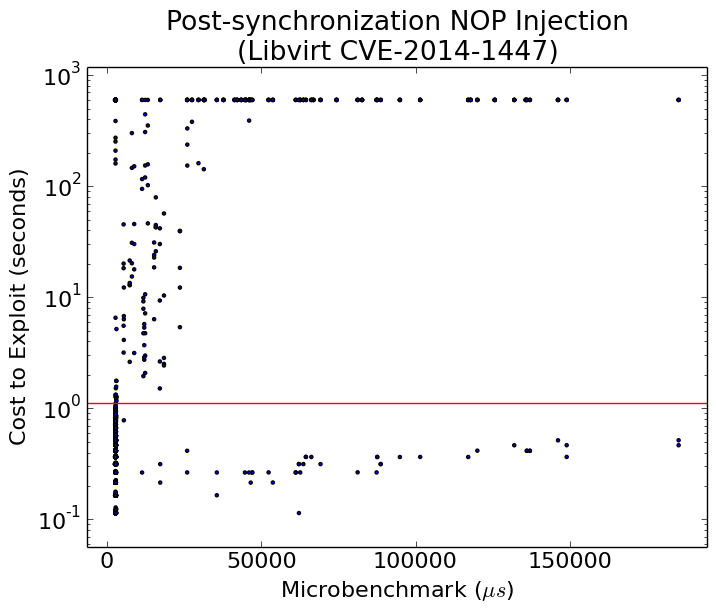
\includegraphics[width=.75\columnwidth]{figures/libvirt-post}
	\caption{
		Exploit cost (in time) as a function of the microbenchmark after applying diversity \textbf{T3} to Libvirt with concurrency bug CVE-2014-1447.
		Beyond microbenchmark measurements of 10 milliseconds, most of exploit costs observed were much greater than the baseline; often the exploit attempts were stopped artificially early and labeled ``failed exploits''.
		This transformation thus increases the average exploit cost with increasing microbenchmark overhead.
	}
	\label{fig_libvirt-post}
\end{figure}

Applying \textbf{T3} to the canonical atomicity violation bug appeared to have negligible effect on exploit cost (Figure \ref{fig_nonatomic-post}). 
\begin{figure}
	\centering
	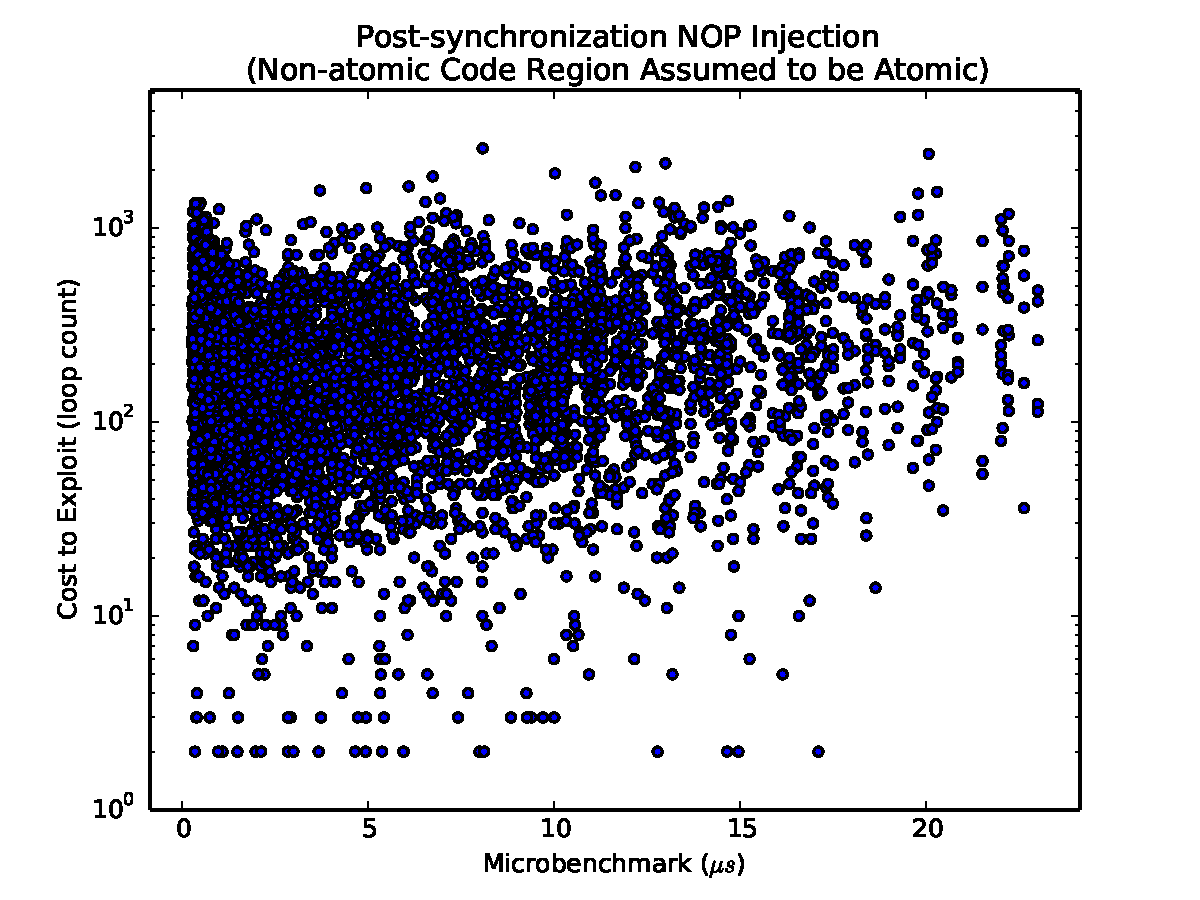
\includegraphics[width=.75\columnwidth]{figures/nonatomic-post}
	\caption{
		Exploit cost (in number of exploit attempts) as a function of the microbenchmark after applying \textbf{T3} to a canonical ``nonatomic-operations-assumed-to-be-atomic'' concurrency bug.
		This transformation does not appear to have an effect on exploit cost for this bug.
	}
	\label{fig_nonatomic-post}
\end{figure}


\section{Discussion \& Future Directions}
It is clear from these results that, at the very least, time randomization increases the exploitation cost for some concurrency bugs.
Then the major argument against employing it universally becomes performance overhead.
While overheads on effective randomizations were unacceptably high using the NOP injection implementations tested here (at least 12x for \textbf{T1} and at least 5x for \textbf{T3}), it is not clear that significant overhead is necessary for time randomization in general.
Part of the effect of time randomization via NOP injection is to modify thread interleavings by signaling with NOPs to the scheduler that another thread can be scheduled.
The randomization between and among threads achieved here with NOP injection could conceivably be achieved directly in the scheduler via random synchronization schedules.
By modifying the scheduler directly, it may be possible to obtain the same benefits shown here with minimal overhead.

Alternatively, a more complicated heuristic could be applied to the garbage code insertion implementations investigated here.
More specifically, for each randomization, measurements could be taken of the extent to which relative thread timing has been randomized, and of some performance metric.
These measurements could be used to decide whether to keep a specific randomization or generate a new one, as well as to calibrate randomization parameters like max delay in this work.

\section{Related Work}
Automated software diversity as a defense strategy has been systematized by Larsen et al.~\cite{Larsen2014}.
That work proposes a taxonomy of cyberattacks and a taxonomy of defenses against those classes of attacks, and surveys many of the studied and unstudied diversification techniques.
To our knowledge, ours is the first work to investigate automated software diversity specifically as it pertains to concurrency attacks.

NOP injection, also known as ``garbage code insertion'', has been investigated many times.
Cohen~\cite{Cohen1993} and Forrest et al.~\cite{Forrest1997} proposed garbage code insertion as a method for diversifying operating system source code as a way to drive up the required complexity of attacks on systems.
Jackson et al. proposed NOP insertion as a diversification technique to be used by a compiler in automatically diversifying programs~\cite{Jackson2011}.

In perhaps the most pertinent related work, Jackson et al. later 

\section{Conclusion}
We have presented time randomization, a subset of automated software diversity which randomizes the timing between and among threads, with the goal of thwarting concurrency attacks which benefit from predictability in that timing.
Our experiments show that at least one of the time randomization transformations tested have a significant effect on the cost to exploit two real-world concurrency bugs.
We believe that transformations with lesser performance costs are worth studying as a defense against concurrency attacks.

%\section*{Acknowledgement}
%This research was supported, in part, by DARPA CRASH.

%
% ---- Bibliography ----
%
{\footnotesize \bibliographystyle{acm}
\bibliography{references}}

\end{document}
